\documentclass[a4paper,11pt]{article}
\usepackage[utf8]{inputenc}
\usepackage[T1]{fontenc}
\usepackage[french]{babel}
\usepackage{textcomp}
\usepackage{listings}
\usepackage{pdfpages}
\usepackage{array}

\title{PROJET\\ UE Méthodes de ranking et recommandations\\ 
		Sujet 5 : Simulation d'un Google Bombing}
\author{Maxime Gonthier - Laureline Martin}

\begin{document}

\pagenumbering{gobble}\clearpage
	\pagenumbering{gobble}\clearpage
	\maketitle
	\newpage\clearpage\pagenumberi ng{arabic}

\newpage
\tableofcontents

\newpage
\section{Introduction}
	Le but de ce projet est de simuler, d'évaluer et de proposer la méthode la plus efficae pour un Google Bombing. Il s'agit d'une technique d'attaque sur le graphe du web afin d'augmenter la pertinence d'une page cible. Pour cela, plusieurs attaquants créent des pages et y insèrent des liens vers une page cible à attaquer. Plusieurs structures de pages attaquantes sont possibles :
	\begin{itemize}
		\item seul
		\item complet
		\item anneau
		\item arbre
	\end{itemize}
	Nous allons tester ces différentes structures sur des pages de pertinences différentes et déterminer quelle est la structures la plus avantageuse pour obtenir la pertinence la plus forte possible.

\section{Manuel utilisateur}
	Notre application se lance grâce à la commande \texttt{make} suivie de fichier ".txt" à modifier.

\section{Plan}
	Dans un premier temps nous allons effectué des tests simples en utilisant quatre type de structures différentes ainsi que trois cibles de pertinences différentes.
	Nous en déduirons des hypothèses sur l'eficacité de chaque structure et l'impact de la pertinence de la cible sur cette même efficacité.
	Dans un second temps nous étudierons l'impact sur la pertinence de graphes générés en nombre aléatoire pour étudier qu'elle structure est globalement la plus efficace.
	Puis nous testerons la meme choses avec cette fois ci un graphe dont les arcs le reliant a lui meme sont générées aléatoirement.
	Enfin nous ferons varier le nombre de sommets du graphe ataquant pour en déduire son efficacité et nous conclurons.
	
\section{I.	Tests initiaux et hypothèses}
	L'algorithme power calculant les pertinences est contenu dans le fichier $ranking.c$. Il n'est pas détaillé dans ce rapport mais le fichier est commenté.
	On considère ici le graphe du web Stanford.txt. Ce graphe est modifié par l'ajout de sommets et d'arcs afin d'augmenter la valeur d'un sommet ciblé.\\
	On considère que :\\
	\begin{itemize}
		\item Les sommets représentent les pages du web.
		\item Les arcs représentent les liens dirigeant vers d'autres pages.
		\item Les valeurs des sommets représentent les pertinences calculés par l'algorithme pagerank.
		\item Le sommet cible représente la page dont on souhaite augmenter la pertinence.
		\item 100 sommets sont ajoutés pour chaque test.
	\end{itemize}
	\subsection{Explications du code}
	A faire.

	\subsection{Résultats des tests initiaux}
		\subsubsection{Stanford.txt sans modification}
			281903 pages\\
			2312497 liens\\
			132 itérations\\
			27.627466 secondes\\
			\\
			Voici les pertinences de base des trois sommets étudiés :\\
			Pertinence forte : Page 280545 - 9.96199e-05\\
			Pertinence moyenne : Page 281466 - 7.53954e-06\\
			Pertinence faible : Page 281574 - 6.05222e-07\\
			\\
		\subsubsection{Résultats}
			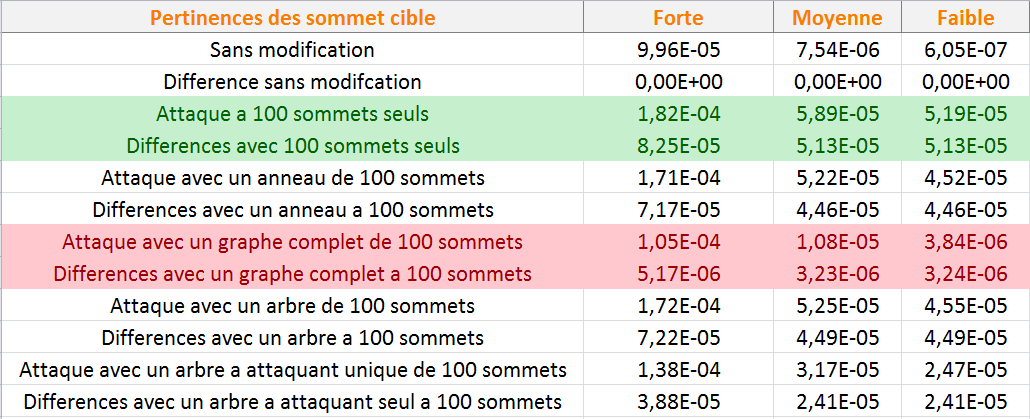
\includegraphics[scale = 0.5]{Captures/ranking1.PNG}

		\subsubsection{Analyses}
		A faire.
			
		\subsubsection{Hypothèses}
		A faire.
			
	\subsection{Conclusion des tests initiaux et hypothèses}
		Cinq structures différentes sont ajoutées : des sommets seuls, un graphe complet, un anneau, un arbre et un arbre a attaquant unique. L'arbre a attaquant unique est un arbre dont seul le sommet racin est relié 
		à la cible. L'objectif de cette structure est de minimiser le nombre de sommets reliées a la cible pour ainsi minimiser les chances de se faire repérer lors de l'attaque.\\
		On observe pour chaque cible que la structure la plus efficace est le sommet seul, suivis de l'arbe, de l'anneau, de l'arbre a attaquant unique et enfin du graphe complet.\\
		La raison de cette ordre serait que pour des sommets seuls, la probabilité de pointer sur la cible est de 1/1 alors qu'elle est de 1/n pour un graphe complet
		avec n le nombre de sommets. Ainsi la probabilité est dilué et donc la cible en sera moins modifié.\\
		On observe que pour chaque structure la différence de modification de la pertinence est presque identique entre les cibles faibles et moyennes.
		Ainsi on peut en déduire que modifier la pertinence d'une cible à e-06 ou e-07 est de même difficulté.\\		
		Pour le sommet sommet seul on observe que la modification de pertinence (la différence) pour une cible forte, moyenne ou faible sont respectivements
		8.25e-05, 5.13e-05 et 5.13e-05. Ainsi on peut en déduire que modifier la pertinence est plus significatif quand la cible est déjà forte.
			
		\subsubsection{Hypothèses}
			On suppose que les structures les plus efficaces sont les sommets seuls et les arbres. On suppose que changer la pertinence d'une cible devient 
			plus difficile à partir d'une cible de pertinence Xe-05 et que c'est assez identique pour les cibles de pertinences Xe-06 et Xe-07.


\section{II.	Tests avec un nombre de graphes générés aléatoirement}
	Nous allons désormais insérer des graphes générés aléatoirement. Ce qui est aléatoire n'est pas la structure des graphes mais le nombre de garphes générés.\\
	L'objectif de cette démarche est de déterminer quel structure est la plus efficace globalement.\\
	C'est a dire quelle structure influe le plus sur la pertinence quelle que soit la situation.\\
	De plus les resultats nous aiderons aussi a determiner l'impact qu'a une certaine structure sur la cible de manière plus générale 
	que dans les cas prédéfinis de la partie précedente.
	Le nombre de sommet des graphes ajoutées est fixé a 100.
	La cible est également fixé ainsi que la structure des graphes ajoutées.
	On va par exemple insérez 5 graphes complet de nombre de sommet respectivement : 25, 10, 5, 6 et 4. Tous reliées au sommet cible.
	Dans un premier temps nous allons expliquer le code derrière cette démarche puis nous analyserons les résultats.

	\subsection{Explication du code}
		Tous est dans le fichier $ajoutsommetsattanquants.c$. Les fonctions utilisées sont $ajoutanneaualeatoire$, $ajoutcompletaleatoire$
		et $ajoutarbrealeatoire$. Ces fonctions reprennent en partie le code des trois fonctions presque eponyme décrite précedemment.
		Regardons ce qui a changé. 
		\begin{lstlisting}
	while(nbsommetrestant > 0) {
		nbajout = rand()%(100-nouveausommets);
		if (nbajout <= 3) { nbajout = 3; }
		nbsommetrestant -= nbajout;
		\end{lstlisting}
		$nbajout$ représente le nombre de sommet que l'on va ajouter dans la première structure créer. Il choisis donc un nombre 
		aléatoire entre 0 et 100 car le nombre de sommet total est limité a 100. Si le nombre choisis est inférieur a 3 on le fixe a 3 car créer
		des anneau ou des graphes complets de tailles inférieure a 3 reviens juste a créer des sommets seuls.
		$nbajout$ est enlevé au nombre de sommet restant a ajouter. Puis on lance la construction de la structure comme vu précedemment 
		avec $nbajout$ représentant le nombre de sommets. A la fin de cette itération $nbajout$ reprends un nombre aléatoire qui cette fois
		prend une valeur entre 0 et 100 moins le nombre de sommets ajouté precedement représenté par $nouveausommets$.

	\subsection{Résultats des tests}
		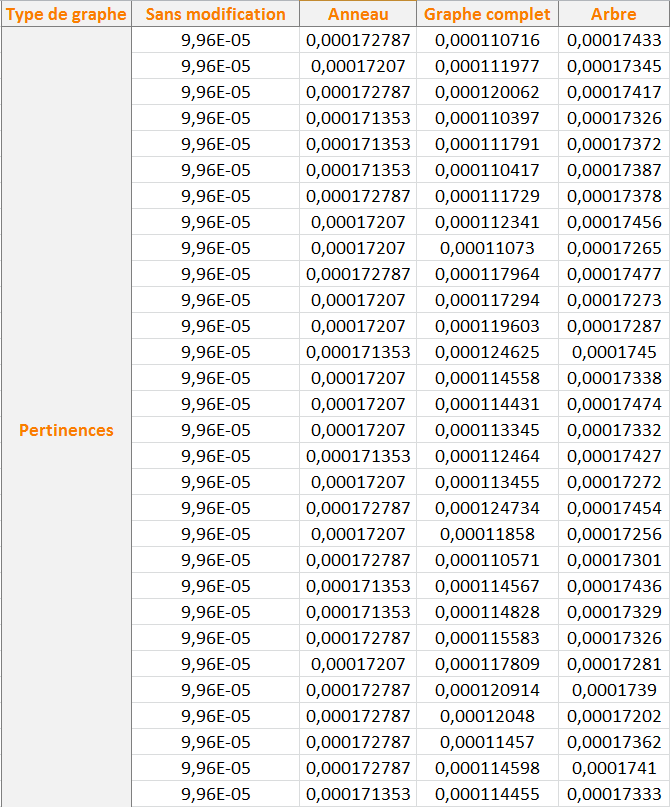
\includegraphics[scale = 0.5]{Captures/ranking2.PNG}\\
		La cible est de pertinence forte. \\
		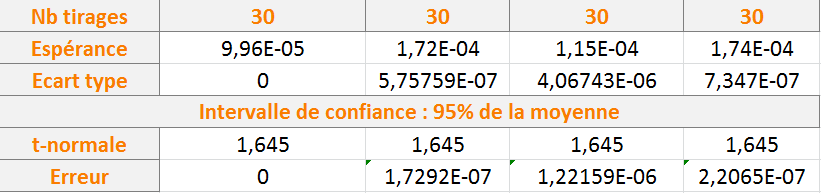
\includegraphics[scale = 0.5]{Captures/ranking3.PNG}\\
		En regardant les espérances on observe que c'est l'anneau est l'abre qui impactent le plus la pertinence de la cible.
		On observe aussi que les erreurs sont inférerieurs à 0,000015 on peut donc faire confiance aux résultats.\\

	\subsection{Analyse graphes en anneau}
		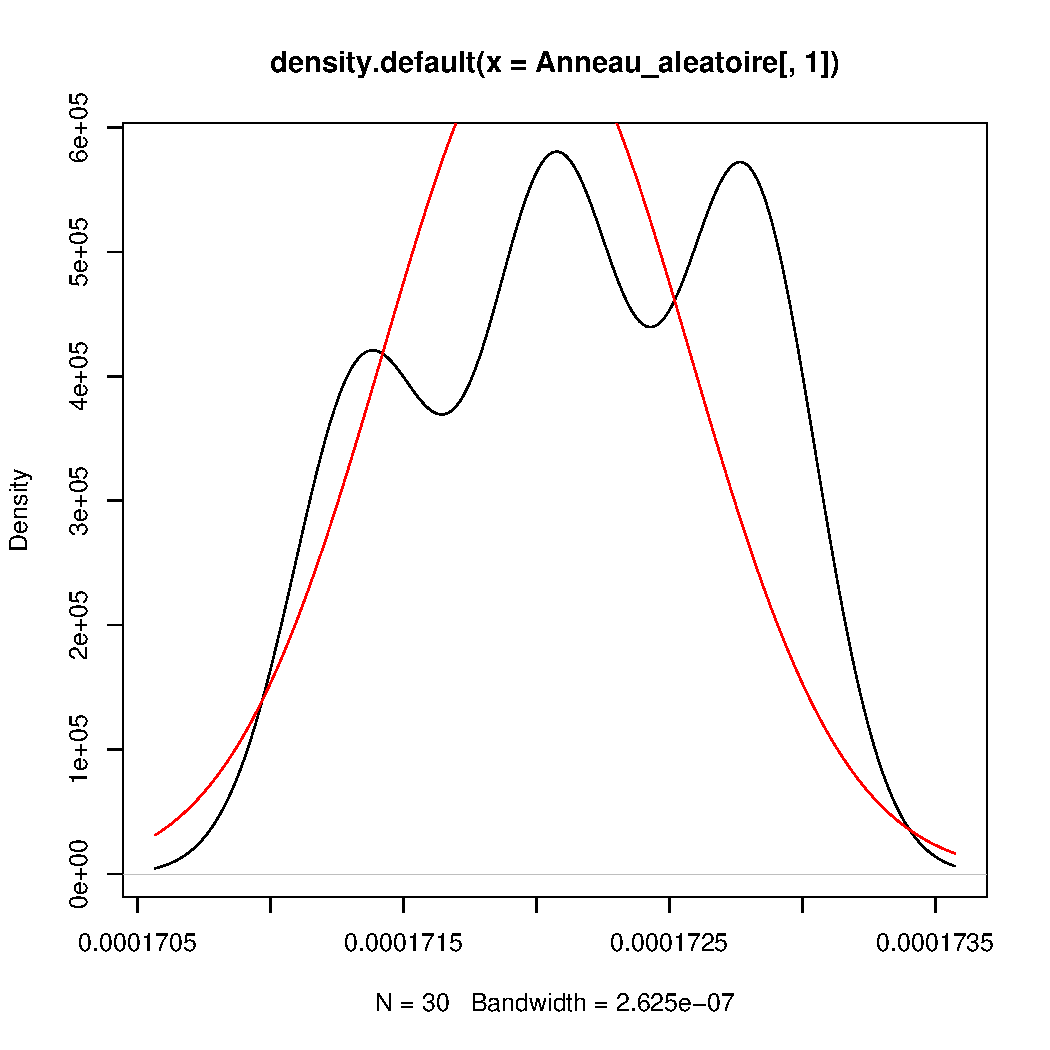
\includepdf{../R/Nombre_de_graphe_aleatoire/Anneau.pdf}
		La courbe rouge représente la loi normale, la noire est la fonction de densité. 

	\subsection{Analyses Graphes complet}
		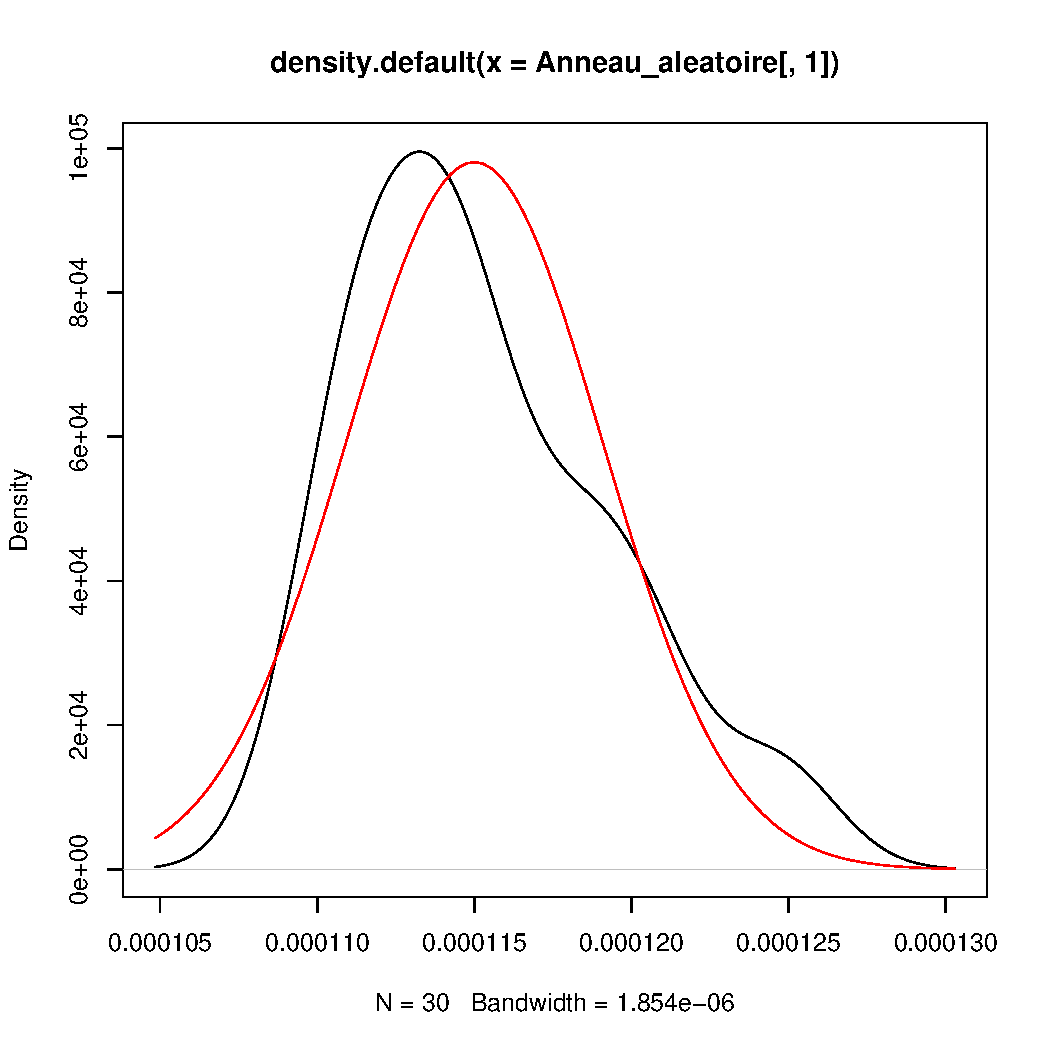
\includepdf{../R/Nombre_de_graphe_aleatoire/Complet.pdf}

	\subsection{Analyses Arbres}
		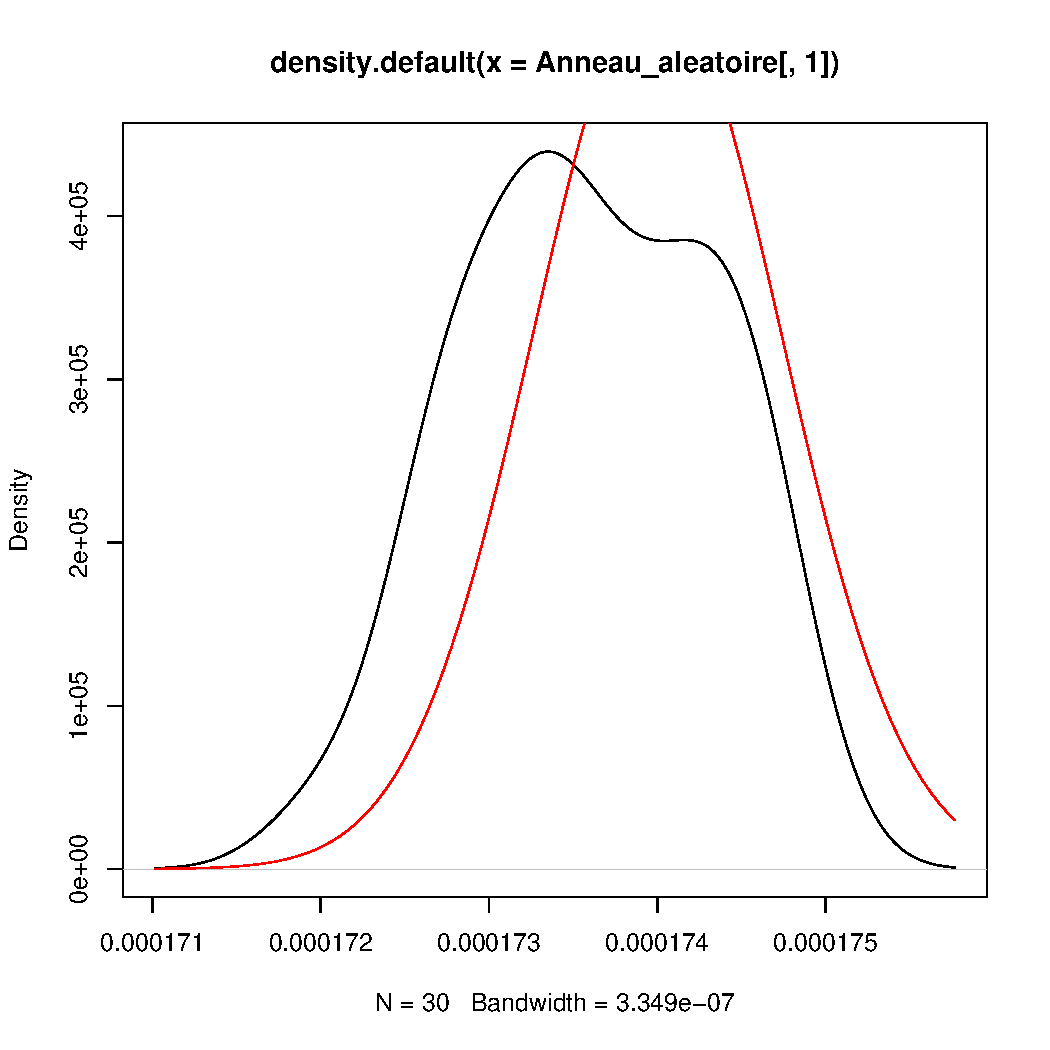
\includepdf{../R/Nombre_de_graphe_aleatoire/Arbre.pdf}

	\subsection{Conclusion sur l'impact de chaque structure}


\section{III.	Expériences avec un graphe de degré aléatoire}
	Ici nous allons créer un graphe de 100 sommets de degré aléatoire. C'est à dire que chaque sommet sera relié au même nombre de sommets au sein du graphe.
	
	\subsection{Résultats des tests}
		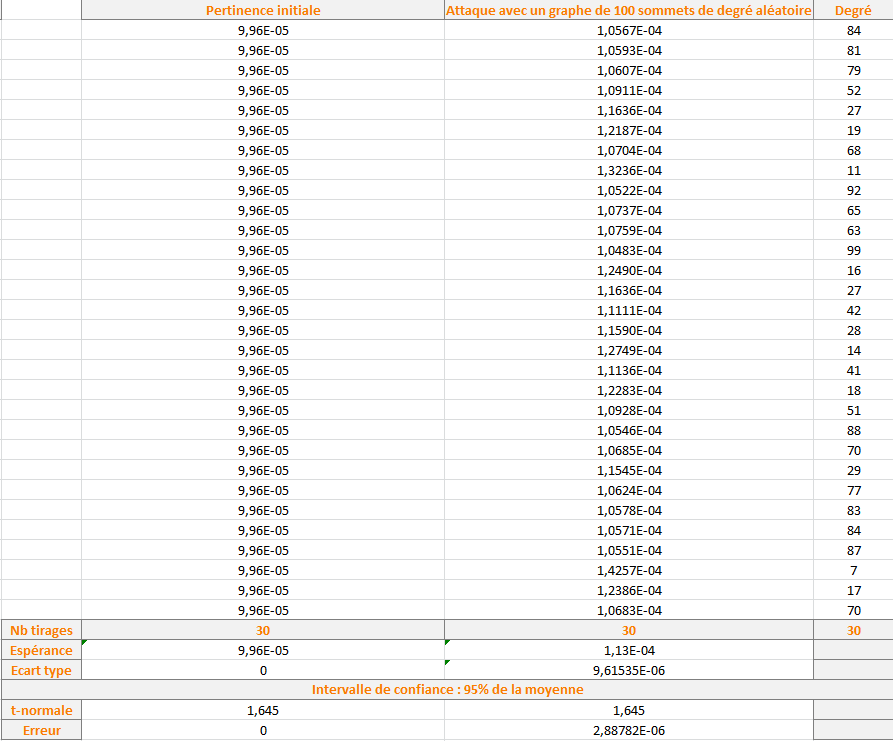
\includegraphics[scale = 0.5]{Captures/ranking4.PNG}\\
		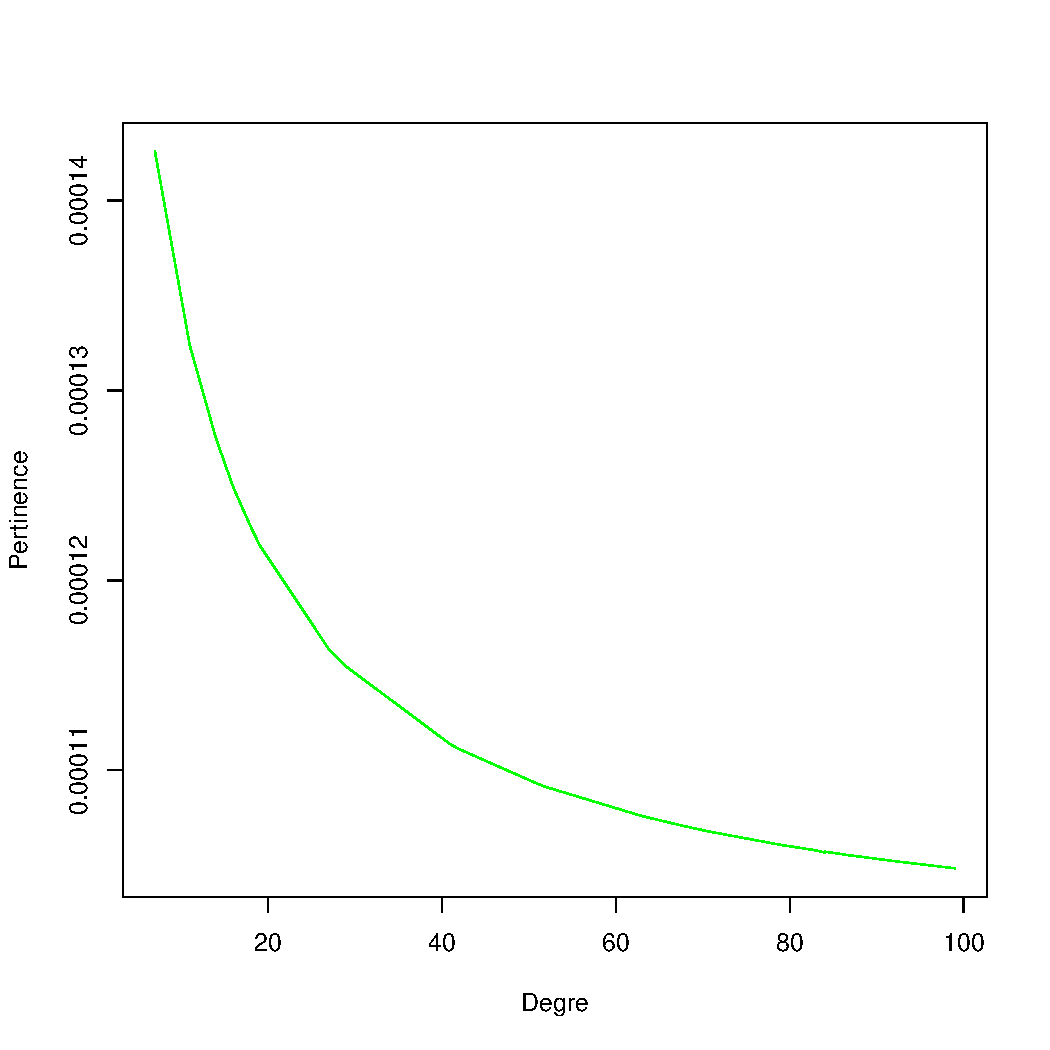
\includepdf{../R/Degre_aleatoire/degre.pdf}
	
	\subsection{Analyses}
		On observe que plus le degré est fort, moins la pertinence de la cible est modifié. Ici l'espérance de la pertinence de la cible apres attaque est de 1.13e-04, ce qui est 
		meilleur que la pertience de la cible lors des tests initiaux avec un graphe complet a 100 sommets (1.05e-04). Ainsi cette structure est plus eficace que le graphe complet.
		De plus cette structure a l'avantage d'etre moins detectable que l'anneau ou le graphe complet car le degré varie. En effet détecter un anneau ou un graphe complet est beaucoup plus aisé 
		que de détecter un graphe de degré X.
	
\section{IV.	Expériences sur l'efficacité}
	
	\subsection{Résultats des tests}
		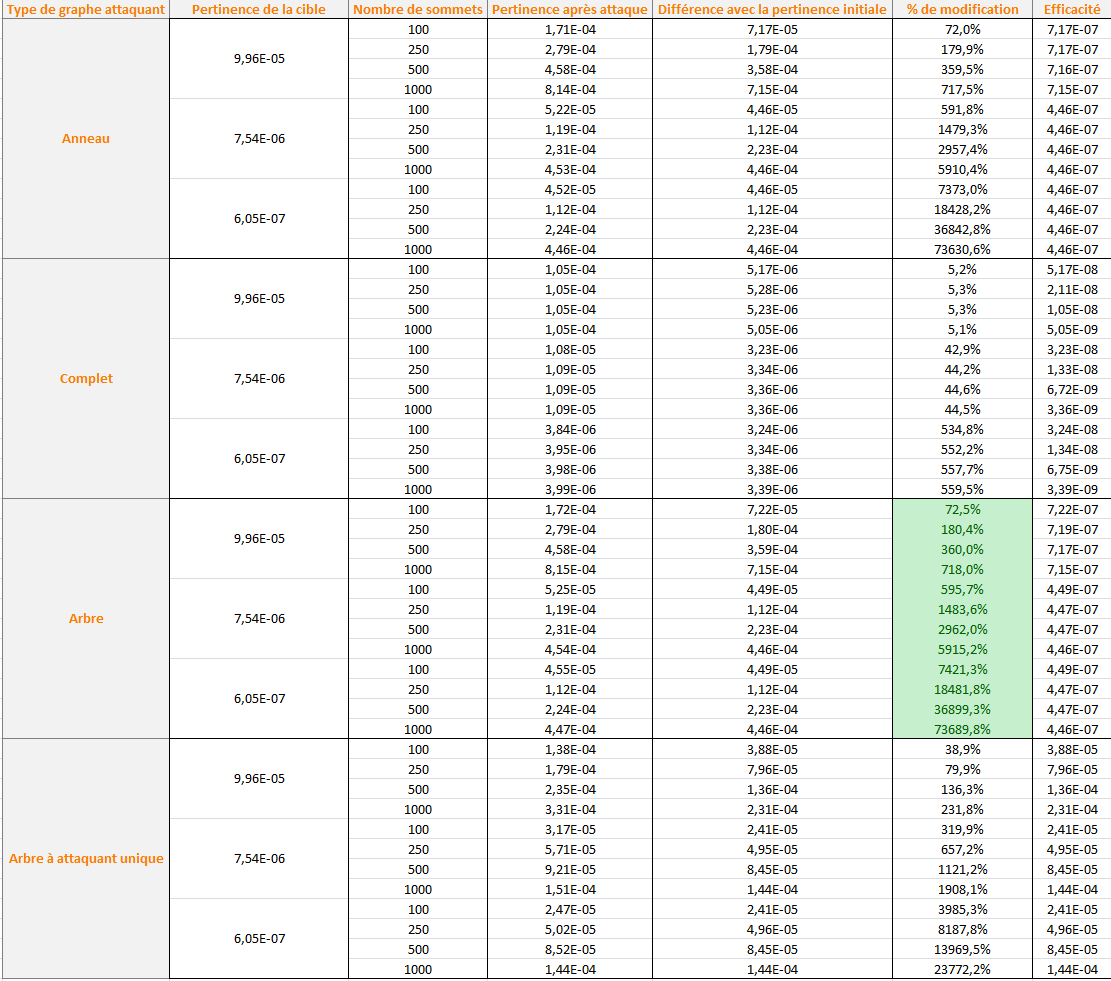
\includegraphics[scale = 0.6]{Captures/ranking5.PNG}\\
	
	\subsection{Analyses}
		Ici nous av
	
\section{Conclusions}

\end{document}
